\section{Data and Embodiment Signals}\label{sec:data}
\subsection{In-vivo robotic video with robot logs}
We use the SurgVU corpus \cite{surgvu}: 155 porcine training-laboratory cases recorded on da Vinci Xi systems, 280 video files totalling 837.8\,h at $1280\times720$ and 60\,fps. Each case comes with the system log of its four universal surgical manipulators (USM1--4): install and uninstall times of every instrument \emph{and of the endoscope}, and with task segments from a training curriculum (218\,h annotated; 7 tasks, 46 curriculum topics). After removing black, out-of-body and blank footage, about 604\,h are usable (Fig.~\ref{fig:pipeline}). Cases are split into 123 training, 12 validation and 20 test cases, stratified by endoscope arm, case length and dominant task.

The logs record part-relative times; converted to a single case timeline they give, at every instant, the robot configuration $s_t=(o^1_t,\dots,o^4_t)$ with $o^k_t$ the occupant of arm $k$ (empty, endoscope, or one of 20 instrument types). The endoscope arm never changes within a case (USM2 in 142 cases, USM3 in 11); three instruments are mounted 65\,\% of the time and instruments are exchanged 7.1 times per hour. The logs are noisy: 97\,\% of overlapping intervals on one arm are stale intervals left by missing uninstall events, which we resolve by letting the most recent installation win.

\subsection{Console overlay}
The surgeon console renders a status band over the recorded video on 81\,\% of usable frames. Per arm it shows the mounted instrument, the endoscope, the hand (left/right) that currently drives the arm, and energy activation. We crop the band away before the model sees any pixel, so that the model cannot read instrument identities from the screen, and use the overlay only as a source of conditioning and evaluation labels.

\begin{figure*}[t]
\centering
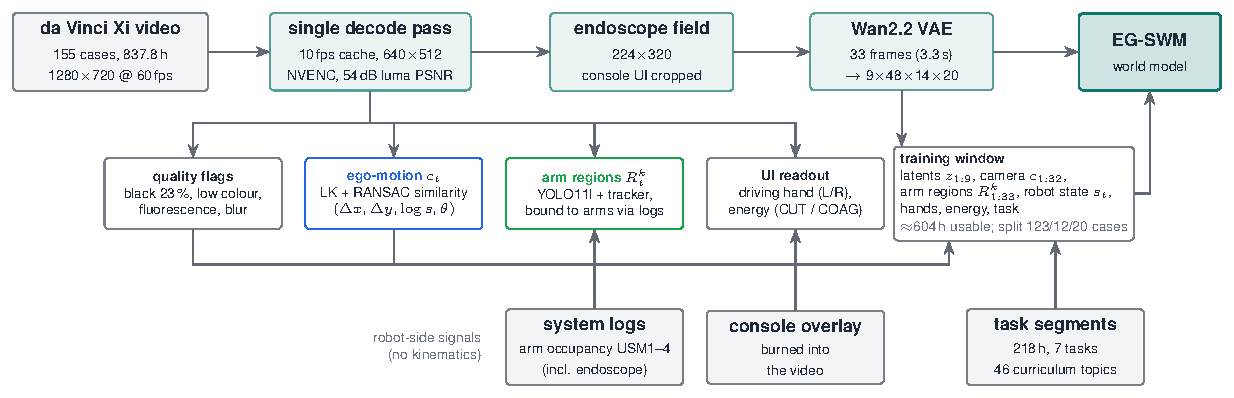
\includegraphics[width=\textwidth]{pipeline.pdf}
\caption{Data pipeline. One decode pass converts the in-vivo video into a 10\,fps cache with per-frame quality flags and endoscope ego-motion; instrument detections are bound to robot arms through the system log; the world model sees only the endoscope field encoded by a frozen video VAE.}
\label{fig:pipeline}
\end{figure*}
